\problemname{Walkways}
\noindent
The Swedish team for the International Olympiad in Informatics has just landed in Singapore to compete in IOI 2020.
On the way to the baggage claim, they have to pass through a long corridor with several moving walkways.
The corridor is $M$ meters long, and the team is currently at the beginning of it, trying to figure out how quickly
they can reach the baggage claim. There are $N$ moving walkways in the corridor. Each walkway starts at a certain
distance from the beginning of the corridor, ends at a certain distance from the beginning of the corridor, and
takes a certain amount of time to travel along. All walkways move in the direction of the corridor, and one can
only step onto a walkway at the beginning of it and step off at the end of it. When the team is not on any walkway,
it takes $g$ seconds to walk one meter. The corridor and walkways are narrow enough that only the time it takes to
travel parallel to the corridor matters. Therefore, if one walkway ends at the same distance from the beginning as
another walkway starts, it takes no time to move between the walkways. If the team plan their route optimally, how
fast can they reach the end of the corridor?

Note that it may be advantageous to sometimes walk backward through the
corridor to reach a walkway that takes one further ahead. However, there are no walkways going backward through the corridor.

\section*{Input}
The first line of input contains three integers $N, M$ and $g$ ($1 \le N \le 2 \cdot 10^5$, $2 \le M \le 2 \cdot 10^5$, $1 \le g \le 100$),
the number of walkways, the length of the corridor in meters and the speed of the team in seconds per meter.

The following $N$ lines each contain three integers describing a walkway, $s_i, e_i$ and $t_i$ 
($1\leq s_i < e_i\leq M,1\leq t_i\leq100$), the number of meters from the start of the corridor to the start of the walkway,
the number of meters from the start of the corridor to the end of the walkway and how long it takes to use the walkway.

\section*{Output}
Print an integer: how long it will take for the team to reach the end of the corridor if they plan their route optimally.

\section*{Points}
Your solution will be tested on several test case groups.
To get the points for a group, it must pass all the test cases in the group.

\noindent
\begin{tabular}{| l | l | p{12cm} |}
  \hline
  \textbf{Group} & \textbf{Point value} & \textbf{Constraints} \\ \hline
  $1$   & $8$      & $N,M \le 10$ and you never have to go backwards. \\ \hline
  $2$   & $13$     & $N,M \le 1000$ and you never have to go backwards. \\ \hline
  $3$   & $40$     & You never have to go backwards. \\ \hline
  $4$   & $15$     & $N,M \le 1000$ \\ \hline
  $5$   & $24$     & No further constraints. \\ \hline
\end{tabular}


\section*{Explanation of Samples}

\begin{figure}[h]
	\centering
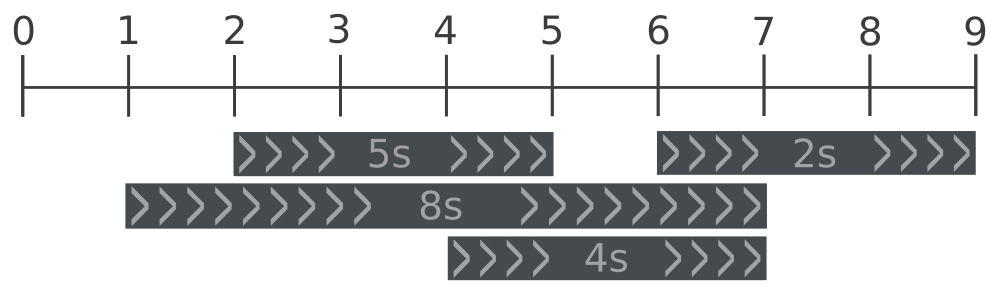
\includegraphics[width=0.7\textwidth]{sample1}
\caption{Sample 1}
\end{figure}
In sample 1, it takes 2 seconds to walk one meter when the team is not on a walkway.
The fastest way to reach the end is to walk to the walkway that takes 5 seconds, use it,
then walk to the walkway that takes 2 seconds and use it.
In total, this takes $4+5+2+2=13$ seconds.




\begin{figure}[h]
	\centering
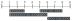
\includegraphics[width=0.7\textwidth]{sample2}
\caption{Sample 2}
\end{figure}
In sample 2, it instead takes 5 seconds to walk one meter when the team is not on a walkway.
The fastest way to reach the end is to walk to the walkway that takes 8 seconds, use it, and then go back
one meter to use the walkway that takes 2 seconds, and then walk the final meter.
In total, this takes $5+8+5+2+5=25$ seconds.

